%-------------------------------------------------------------------------------
%                            BAB II
%               TINJAUAN PUSTAKA DAN DASAR TEORI
%-------------------------------------------------------------------------------

\chapter{TINJAUAN KEPUSTAKAAN}                

\section{Struktur Penyaluran Gas LPG 3 Kg}
\par Dalam pendistribusian gas elpiji ke masyarakat, sepenuhnya dilakukan oleh Pertamina dengan sistem \textit{close loop  supply chain}, yaitu suatu aliran produk mulai dari konsumen, kembali ke pabrik untuk diproses ulang kemudian kembali lagi ke konsumen sebagai barang baru.
\par Dalam alur distribusi LPG 3 kg, yang pertama adalah berasal dari Depot LPG. Kemudian dari Depot LPG, jalur berikutnya disebut SPPBE (Stasiun Pengisian dan Pengangkutan Bulk LPG ) yang dikelola oleh Pertamina dan pihak swasta, kemudian setelah itu paket LPG diterima oleh agen LPG dan selanjutnya sebagai ujung tombaknya disebut sub agen atau pangkalan LPG. Sub agen LPG inilah yang berhubungan langsung dengan pengecer, warung atau juga konsumen. seperti pada \ref{penyaluran}.
\begin{figure}[H]
	\centering
	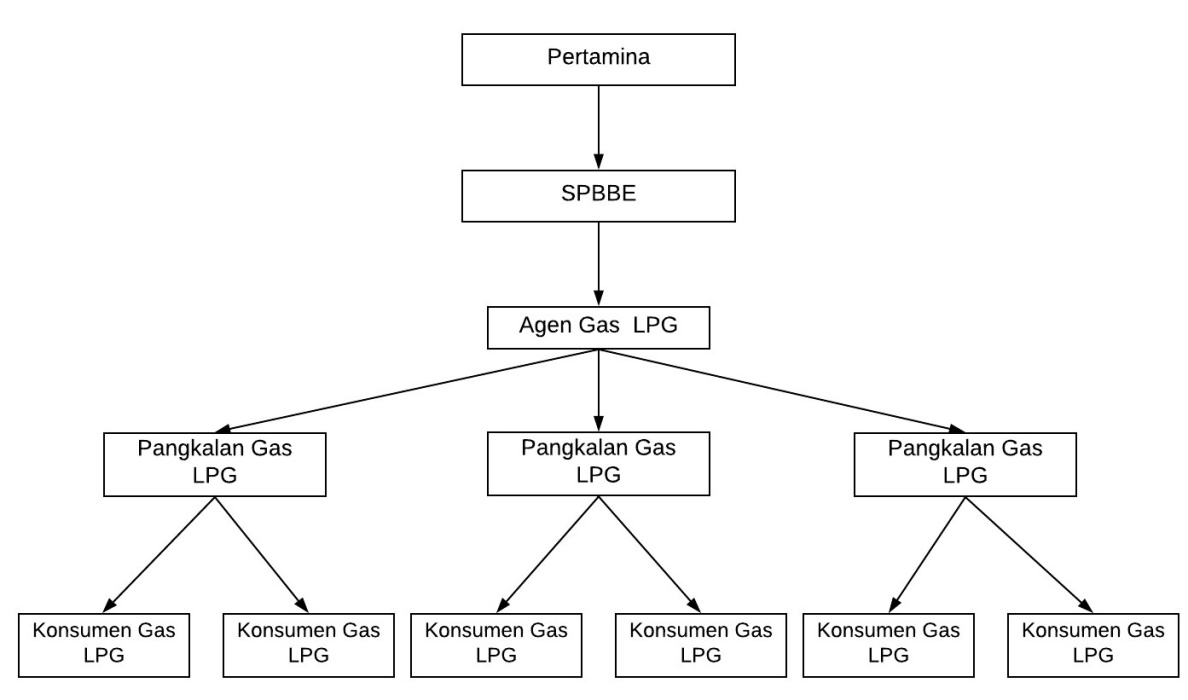
\includegraphics [width = 10cm, height= 10cm]{gambar/struktur-penyaluran}
	\caption{Struktur Penyaluran Gas LPG}
	\label{penyaluran}
\end{figure}


\section{Gas Subsidi LPG 3Kg}
\par Sejak Pemerintah melakukan konversi dari minyak tanah ke gas LPG yang dilakukan sejak tahun 2007. Kebutuhan untuk tabung gas LPG semakin meningkat dan gas subsidi LPG 3 kg yang ditawarkan pemerintah di awal periode konversi, semakin berkurang. Ini dikarenakan jenis tabung ini dianggap lebih ekonomis di bandingkan dengan tabung gas dan banyak rumah tangga dan industri rumahan kecil yang masih memakai tabung gas jenis ini sebagai alat untuk memasak.
\begin{figure}[H]
	\centering
	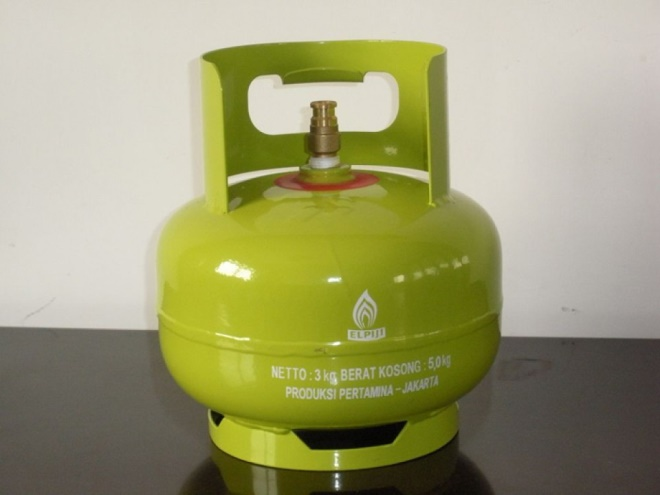
\includegraphics [width = 6cm, height= 8cm]{gambar/tabung-gas}
	\caption{Tabung Gas LPG}
	\label{tabung}
\end{figure}

\par Maka dari itu pertamina selaku distributor telah memberlakukan kebijakan kepada konsumen yang ingin membeli gas subsidi ini harus menunjukkan kartu keluarga (KK) dan Kartu Tanda Penduduk (KTP) sehingga jumlah tabung yang di beli dapat dibatasi berdasarkan KK.

\section{Android}
\par Android merupakan sistem operasi yang dibangun untuk perangkat mobile. Komponen-komponen dari sistem operasi Android ditulis dengan bahasa pemrograman C atau C++, akan tetapi aplikasi pengguna yang digunakan untuk Android ditulis dalam bahasa pemrograman Java \cite{ableson2012android}. Android juga dapat diartikan sebagai sistem operasi perangkat seluler berbasis Linux yang menyediakan run time environment yang disebut dengan \textit{Android Runtime} (ART) yang telah dioptimasi untuk perangkat dengan sistem memori yang kecil. Karena Android merupakan platform open source, maka setiap orang bebas untuk membuat dan mengembangkan suatu aplikasi \cite{supardi2011}.
\begin{figure}[H]
	\centering
	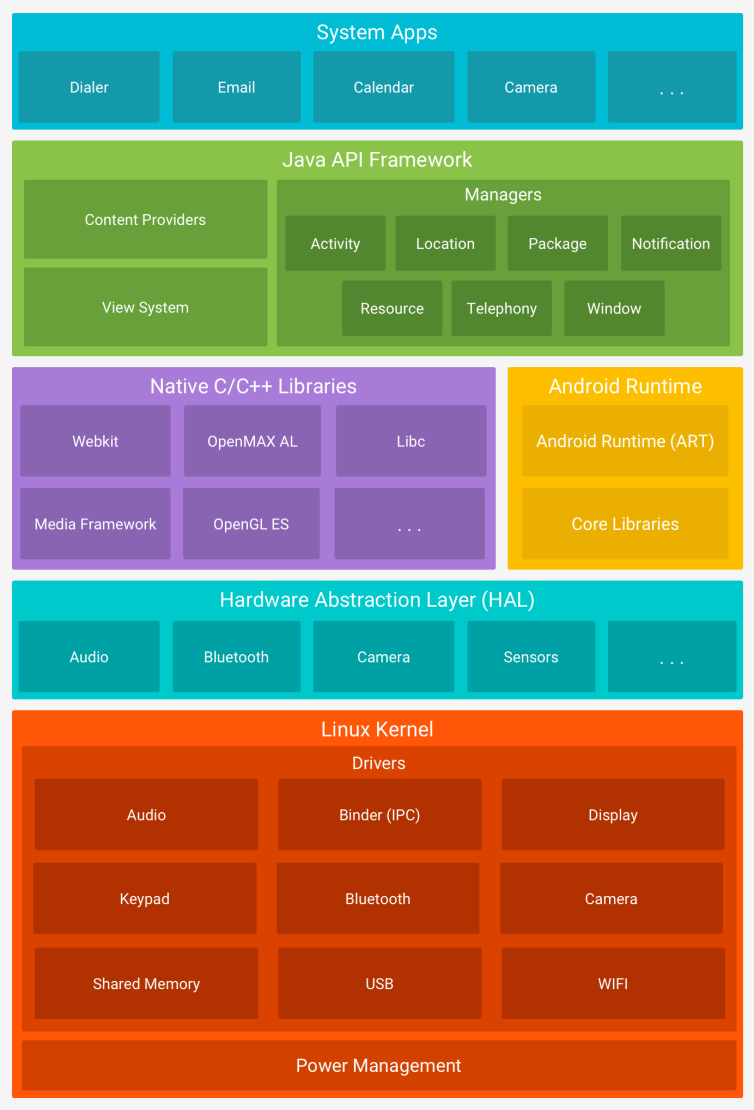
\includegraphics [width = 7cm, height= 6cm]{gambar/android}
	\caption{Logo Android}
	\label{android}
\end{figure}



%-----------------------------------------------------------------------------%

\section{Aplikasi Hybrid (\textit{Mobile Hybrid App})}
Aplikasi hybrid adalah aplikasi web yang ditransformasikan menjadi kode native pada platform seperti iOS atau Android. Aplikasi hybrid biasanya menggunakan browser untuk mengijinkan aplikasi web mengakses berbagai fitur di device mobile seperti Push Notification, Contacts, atau Offline Data Storage. Beberapa tools untuk mengembangkan aplikasi hybrid antara lain Phonegap, Rubymotion dan lain-lain \textit{\cite{Permana}}.
\begin{figure}[H]
	\centering
	\fbox{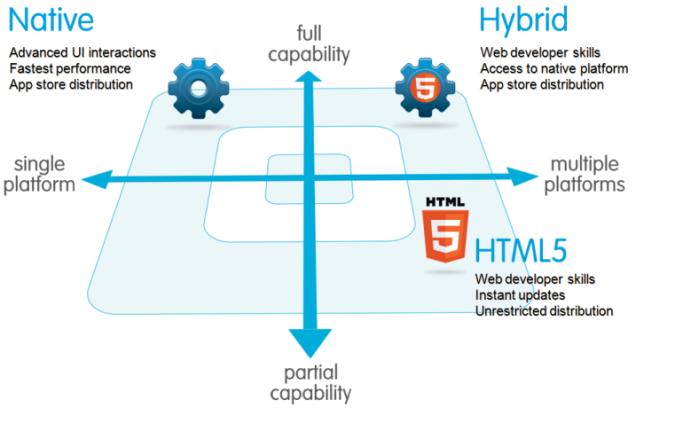
\includegraphics [width = 12cm, height= 8cm]{gambar/hybrid}}
	\caption{Perbandingan Aplikasi Native \& Hybrid}
	\label{android}
\end{figure}
\par Keuntungan membangun aplikasi hybrid diantaranya pemeliharaan project menjadi semakin mudah jika dibandingkan dengan aplikasi native. Aplikasi hybrid juga, bisa dibangun secara cepat untuk keperluan cross platform dan dana yang bisa menjadi lebih hemat jika dibandingkan dengan native.


\section{Ionic Framework}

Ionic adalah \textit{framework front-end} yang dikhususkan untuk membangun aplikasi \textit{hybrid} dengan HTML5, CSS dan AngularJS. Ionic menggunakan Node.js SASS, AngularJS sebagai \textit{engine}-nya. Ionic dilengkapi dengan komponen-komponen CSS seperti \textit{button, list, card, form, grids, tabs}, dan masih banyak lagi. Jadi Ionic itu merupakan teknologi web yang bisa digunakan untuk membuat suatu aplikasi \textit{mobile}. Karena \textit{hybrid} maka aplikasi hanya dibuat satu kali tetapi sudah bisa dirilis di lebih dari satu \textit{platform} dengan kata lain \textit{cross-platform} \textit{\cite{Wahyuni}}.


\section{Apache Cordova}
\par Seperti yang telah dijelaskan di atas, bahwa Ionic hanya menyediakan \textit{framework Front-end} sedangkan untuk mengubahnya ke dalam \textit{platform} Android dan IOS, Ionic menggunakan Apache Cordova. Apache Cordova adalah \textit{platform} untuk membangun aplikasi \textit{mobile native} menggunakan HTML, CSS dan JavaScript. Native mobile application yang didukung antara lain Android, iOS, Windows Phone dan Blackberry.
\par Apache Cordova berisi sekumpulan API (\textit{Application Programming Interface}) untuk mengakses device dari perangkat mobile. Device itu antara lain kamera, GPS (\textit{Global Positioning System}), storage dan lain-lain.  Dengan menunggunakan UI (\textit{User Interface}) framework seperti jQuery Mobile, Dojo Mobile atau Sencha Touch, maka kita dapat mengakses API ini. Dengan kata lain kita dapat membangun aplikasi hanya menggunakan HTML, CSS dan Javascript.


\section{Angular}
\par Untuk melakukan implementasi logika, Ionic menggunakan teknologi framework javascript bernama Angular yang menawarkan performa dan respon cepat seperti aplikasi \textit{native}. sebelumnya dikenal dengan nama AngularJS, sekarang dikenal dengan nama Angular (tanpa JS dibelakang). Angular yang merupakan versi terkini dari AngularJS tentu masih banyak peminatnya di dunia pemrograman. Angular telah mengalami banyak sekali perubahan dibandingkan pendahulunya AngularJS. Angular kini sudah side by side dengan framework Javascript modern lainnya seperti React, Vue dan lain-lainnya. Secara konsep Angular sudah lumayan matang, dengan mampu mengakomodir component based dan dengan bergabungnya Typescript milik Microsoft dan RxJS milik ReactiveX untuk mendukung kemapanan framework ini. Performa yang dihasilkan oleh Angular kini bisa disejajarkan dengan para kompetitor dikelasnya.


\section{\textit{Extreme Programming} (XP)}
\par eXtreme Programming adalah sebuah model pengembangan sistem yang menyederhanakan berbagai tahapan proses pengembangan agar tercapainya peningkatan efsiensi dan fleksibilitas sebuah proyek pengembangan perangkat lunak. Model \textit{Extreme Programming} ini mengedepankan proses pengembangan yang lebih responsive terhadap kebutuhan klien dibandingkan dengan model- model tradisional lainnya sambil membangun suatu perangkat lunak dengan kualitas yang lebih baik. \textit{Extreme Programming} menawarkan sebuah dispilin baru dalam pengembangan perangkat lunak secara agile. Nilai dasar yang terkandung di dalam eXtreme Programming adalah : komunikasi (\textit{communication}), kesederhanaan (\textit{simplicity}), umpan balik (\textit{feedback}), keberanian (\textit{courage}) dan kualitas kerja (\textit{quality work}). Menurut Pressman dalam bukunya yang berjudul Sofware Engineering, edisi keenam, proses \textit{Extreme Programming} memiliki kerangka kerja yang terbagi menjadi empat konteks aktivitas utama. Empat konteks tersebut adalah \textit{planning, design, coding dan testing}. Keempat aktivitas inilah yang akan menghasilkan sebuah perangkat lunak yang didasari dengan konsep.
\begin{figure}[H]
	\centering
	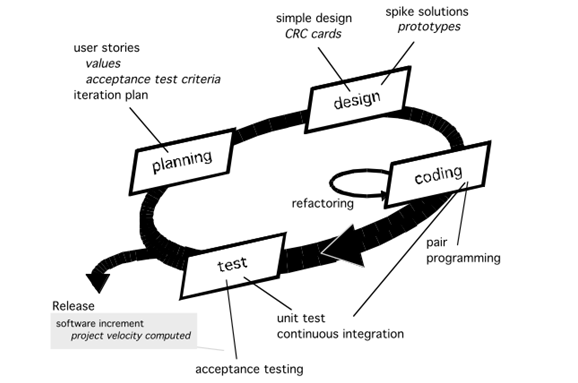
\includegraphics [width= 12cm, height= 10cm]{gambar/xp}
	\caption{Aktivitas Utama XP}
	\label{xp}
\end{figure}
Dalam pembuatannya XP memiliki beberapa langkah operasional yang harus dilakukan seperti :

\subsection{\textit{Planning}}
Planning atau perencanaan adalah proses yang dirancang untuk mencapai tujuan tertentu dan pengambilan keputusan untuk mencapai hasil yang diinginkan. Kebutuhan yang dibutuhkan pada tahap ini yaitu:
\begin {enumerate} [a.]
\itemsep0em
\item Teknik pengumpulan data
\item Analisis kebutuhan sistem
\item Identifikasi aktor
\item Identifikasi use case
\end {enumerate}
\par Aktifitas planning pada model proses XP berfokus pada mendapatkan gambaran fitur serta fungsi dari perangkat lunak yang akan dibangun. Pada aktivitas ini dimulai dengan membuat kumpulan cerita atau gambaran yang diberikan klien yang kemudian akan menjadi gambaran dasar dari perangkat lunak.
\par Kumpulan tersebut nantinya dikumpulkan dalam sebuah indeks cerita dimana setiap poin dari indeks tersebut ditentukan prioritasnya untuk dibangun. Anggota tim dari pengembang aplikasi nantinya akan menentukan alur pengembangan aplikasi dengan terlebih dahulu memulai mengembangkan tugas dengan resiko dan nilai prioritas yang tinggi terlebih dahulu. Dan selutuh tugas akan selesai dalam tenggat waktu dua minggu.
\par Selama proses pengembangan, klien dapat mengubah, memperkecil, membagi dan membuang setiap rencana dari aplikasi. Tim XP akan mempertimbangkan setiap perubahan yang diajukan client berikutnya akan mengubah setiap rencana dari pengembangan perangkat lunak.

\subsection{\emph{Design}}
\par Aktifitas design dalam pengembangan aplikasi bertujuan untuk mengatur pola logika dalam sistem. Sebuah design yang baik dapat mengurangi ketergantungan antar setiap proses pada sebuah sistem. Dengan begitu, jika salah satu fitur pada sistem mengalami kerusakan, tidak akan mempengaruhi sistem secara keseluruhan.
\par Design pada model proses XP menjadi panduan dalam membangun perangkat lunak yang didasari dari cerita client sebelumnya. Dalam XP, proses design terjadi sebelum dan sesudah aktivitas coding berlangsung. Dimana aktivitas design terjadi secara terus-menerus selama proses pengembangan aplikasi berlangsung.

\subsection{\emph{Coding}}
\par Setelah menyelesaikan pengumpulan cerita dan menyelesaikan \textit{design} untuk aplikasi secara keseluruhan, XP lebih merekomendasikan tim untuk terlebih dahulu membuat modul unit tes yang bertujuan untuk melakukan uji coba setiap cerita yang didapat dari klien. Setelah berbagai unit tes selesai dibangun, barulah tim melanjutkan aktivitasnya ke penulisan coding aplikasi. XP menerapkan konsep \textit{pair programming} dimana setiap tugas sebuah modul dikembangkan oleh dua orang programmer. XP beranggapan, 2 orang akan lebih cepat dan baik dalam menyelesaikan sebuah masalah. Selanjutnya, modul aplikasi yang sudah selesai dibangun akan digabungkan dengan aplikasi utama.

\subsection{\emph{Testing}}
\par Tahapan uji coba pada XP sudah dilakukan juga pada saat tahapan sebelumnya yaitu \textit{coding}. Pengujian perangkat lunak dimaksudkan untuk menguji semua elemen-elemen perangkat lunak yang dibuat apakah sudah sesuai dengan yang diharapkan. XP menerapkan perbaikan masalah kecil dengan sesegera mungkin akan lebih baik dibandingkan menyelesaikan masalah pada saat akan mencapai tenggat akhir. Oleh karena itu, setiap modul yang sedang dikembangkan akan terlebih dahulu mengalami pengujian dengan modul unit tes yang telah dibuat sebelumnya.

\subsection{Keunggulan \textit{Extreme Programming}}
\par Keunggulan dari metode pengembangan perangkat lunak \textit{eXtreme Programming} adalah sebagai berikut: \cite{Michael}
\begin{itemize}
	\itemsep0em
	\item Meningkatkan kepuasan kepada klien.
	\item Membangun system dengan lebih cepat.
	\item Menjalin komunikasi yang baik dengan klien.
	\item Meningkatkan komunikasi dan sifat saling menghargai antar developer.
\end{itemize}

\section {\textit{Test Plan}}
\par Test Plan adalah dokumen yang berisi definisi tujuan dan sasaran pengujian dalam lingkup iterasi (atau proyek), item-item yang menjadi target pengujian, pendekatan yang akan diambil, sumber daya yang dibutuhkan dan point untuk diproduksi. Dengan kata lain test plan dapat disebut sebagai perencanaan atau scenario untuk melakukan testing yang akan dilakukan baik oleh expert atau user umum. (Shanardi, 2017)
\par Tujuan umum membuat test plan secara umum adalah untuk memudahkan developer untuk melakukan testing agar testing yang dilakukan menjadi jelas sehingga hasilnya lebih berguna dan efisien. Tentunya dalam proses pembuatan test plan ini memerlukan beberapa langkah seperti berikut :
\begin{itemize}
	\itemsep0em
	\item \textit{Test Plan Identifier}
	\par \textit{Test Plan Identifier} adalah bagian untuk menjelaskan secara singkat mengenai objek yang akan di test. Bisa berupa penjelasan narasi atau berbentuk tabel dengan kategori kategori tertentu. Informasi yang dijelaskan dapat berupa sekilas mengenai subjek testing, nama orang yang bertanggung jawab terhadap testing, penyusun test plan , tanggal dibuat test plan dan tanggal revisi,dll.
	
	\item Introduction
	\par Pada bagian introduction dibuat untuk menjelaskan secara narasi, mengenai testing yang akan dilakukan terhadap suatu objek testing. Bagian Introduction dapat dibuat lebih rinci dengan menambahkan sub bab apabila perlu untuk dibuat. Contoh subbab yang dapat dibuat antara lain :
	\begin{itemize}
		\itemsep0em
		\item \textit{Purpose} : untuk menjelaskan tujuan \textit{testing}  secara spesifik.
		\item \textit{Background} : latar belakang mengapa \textit{testing} dilakukan.
		\item \textit{Scope} : sejauh mana \textit{testing} dilakukan
		\item \textit{Definition and acronyms} : Penjelasan mengenai singkatan dan istilah yang ada di dalam dokumen test plan.
	\end{itemize}
	
	\item \textit{Test Items}
	\par Bagian test item menjelaskan mengenai daftar komponen komponen dalam objek testingyang akan di test satu per Satu.
	
	\item \textit{Features to be tested}
	\par Menjelaskan fitur fitur apa saja yang ada di dalam objek \textit{testing}, namun fitur tersebut tidak akan di test pada saat pelaksanaan \textit{testing} dan disertakan penjelasan singkat mengapa fitur tersebut tidak di test pada saat \textit{testing}.
	
	\item \textit{Item pass / fail criteria}
	\par Berisi tentang kriteria-kriteria yang harus dipenuhi sebelum berlanjut ke fase berikutnya contoh :
	\begin{itemize}
		\itemsep0em
		\item Jika suatu item di test sebanyak 10 kali dan 9 kali diantaranya berhasil namun ada 1 dimana benar benar gagal maka \textit{item} tersebut dinyatakan sebagai gagal/ \textit{fail}.
		\item Jika hasil dari suatu item sama dengan hasil yang diharapkan maka \textit{item} tersebut dinyatakan berhasil/\textit{pass}.
		\item \textit{System Crash} akan dinyatakan sebagai \textit{fail},dsb.
	\end{itemize}
	
	\newpage
	\item \textit{Testing Task}
	\par Menjelaskan kegiatan testing kepada pihak yang akan melaksanakan kegiatan tersebut.
	
	\item \textit{Responsibilities}
	\par Rincian pihak pihak yang akan bertanggung jawab terhadap suatu kegiatan task di dalam serangkaian kegiatan testing yang akan dilaksanakan
	
	\item \textit{Schedule}
	\par Ada beberapa tujuan dalam membuat schedule di dalam test plan, antara lain :
	\begin{itemize}
		\itemsep0em
		\item Merincikan tolak ukur waktu pengerjaan \textit{testing}.
		\item Estimasi waktu yang dibutuhkan untuk setiap \textit{task}.
		\item Menjadwalkan \textit{testing task} dan \textit{test milestone}.
		\item Merincikan periode pemakaian \textit{testing resource}. 
		\cite{Shanardi}
	\end{itemize}
\end{itemize}

\section {\textit{Usability Testing}}
\par Usability Testing atau tes produk merupakan metode riset untuk mengembangkan dan menyempurnakan produk baru maupun yang telah ada. Inti dari riset ini adalah mendudukkan pengguna/pelanggan di pusat, lalu mengambil pelajaran dari sana . maka dalam test ini, mutlak adanya pengamatan secara langsung (Nielsen, 2012)
\par Dengan mendokumentasikan pengalaman aktual para calon pengguna aplikasi / produk dapat dievealuasi , sebab dari uji ini diharapkan akan menangkap kekuatan dan kelemahan dari setiap aspek yang ada pada aplikasi itu sendiri.

%-----------------------------------------------------------------------------%

% Baris ini digunakan untuk membantu dalam melakukan sitasi
% Karena diapit dengan comment, maka baris ini akan diabaikan
% oleh compiler LaTeX.
\begin{comment}
\bibliography{daftar-pustaka}
\end{comment}
